\documentclass[]{article}
\usepackage{lmodern}
\usepackage{amssymb,amsmath}
\usepackage{ifxetex,ifluatex}
\usepackage{fixltx2e} % provides \textsubscript
\ifnum 0\ifxetex 1\fi\ifluatex 1\fi=0 % if pdftex
  \usepackage[T1]{fontenc}
  \usepackage[utf8]{inputenc}
\else % if luatex or xelatex
  \ifxetex
    \usepackage{mathspec}
  \else
    \usepackage{fontspec}
  \fi
  \defaultfontfeatures{Ligatures=TeX,Scale=MatchLowercase}
\fi
% use upquote if available, for straight quotes in verbatim environments
\IfFileExists{upquote.sty}{\usepackage{upquote}}{}
% use microtype if available
\IfFileExists{microtype.sty}{%
\usepackage{microtype}
\UseMicrotypeSet[protrusion]{basicmath} % disable protrusion for tt fonts
}{}
\usepackage[margin=1in]{geometry}
\usepackage{hyperref}
\hypersetup{unicode=true,
            pdfborder={0 0 0},
            breaklinks=true}
\urlstyle{same}  % don't use monospace font for urls
\usepackage{color}
\usepackage{fancyvrb}
\newcommand{\VerbBar}{|}
\newcommand{\VERB}{\Verb[commandchars=\\\{\}]}
\DefineVerbatimEnvironment{Highlighting}{Verbatim}{commandchars=\\\{\}}
% Add ',fontsize=\small' for more characters per line
\usepackage{framed}
\definecolor{shadecolor}{RGB}{248,248,248}
\newenvironment{Shaded}{\begin{snugshade}}{\end{snugshade}}
\newcommand{\AlertTok}[1]{\textcolor[rgb]{0.94,0.16,0.16}{#1}}
\newcommand{\AnnotationTok}[1]{\textcolor[rgb]{0.56,0.35,0.01}{\textbf{\textit{#1}}}}
\newcommand{\AttributeTok}[1]{\textcolor[rgb]{0.77,0.63,0.00}{#1}}
\newcommand{\BaseNTok}[1]{\textcolor[rgb]{0.00,0.00,0.81}{#1}}
\newcommand{\BuiltInTok}[1]{#1}
\newcommand{\CharTok}[1]{\textcolor[rgb]{0.31,0.60,0.02}{#1}}
\newcommand{\CommentTok}[1]{\textcolor[rgb]{0.56,0.35,0.01}{\textit{#1}}}
\newcommand{\CommentVarTok}[1]{\textcolor[rgb]{0.56,0.35,0.01}{\textbf{\textit{#1}}}}
\newcommand{\ConstantTok}[1]{\textcolor[rgb]{0.00,0.00,0.00}{#1}}
\newcommand{\ControlFlowTok}[1]{\textcolor[rgb]{0.13,0.29,0.53}{\textbf{#1}}}
\newcommand{\DataTypeTok}[1]{\textcolor[rgb]{0.13,0.29,0.53}{#1}}
\newcommand{\DecValTok}[1]{\textcolor[rgb]{0.00,0.00,0.81}{#1}}
\newcommand{\DocumentationTok}[1]{\textcolor[rgb]{0.56,0.35,0.01}{\textbf{\textit{#1}}}}
\newcommand{\ErrorTok}[1]{\textcolor[rgb]{0.64,0.00,0.00}{\textbf{#1}}}
\newcommand{\ExtensionTok}[1]{#1}
\newcommand{\FloatTok}[1]{\textcolor[rgb]{0.00,0.00,0.81}{#1}}
\newcommand{\FunctionTok}[1]{\textcolor[rgb]{0.00,0.00,0.00}{#1}}
\newcommand{\ImportTok}[1]{#1}
\newcommand{\InformationTok}[1]{\textcolor[rgb]{0.56,0.35,0.01}{\textbf{\textit{#1}}}}
\newcommand{\KeywordTok}[1]{\textcolor[rgb]{0.13,0.29,0.53}{\textbf{#1}}}
\newcommand{\NormalTok}[1]{#1}
\newcommand{\OperatorTok}[1]{\textcolor[rgb]{0.81,0.36,0.00}{\textbf{#1}}}
\newcommand{\OtherTok}[1]{\textcolor[rgb]{0.56,0.35,0.01}{#1}}
\newcommand{\PreprocessorTok}[1]{\textcolor[rgb]{0.56,0.35,0.01}{\textit{#1}}}
\newcommand{\RegionMarkerTok}[1]{#1}
\newcommand{\SpecialCharTok}[1]{\textcolor[rgb]{0.00,0.00,0.00}{#1}}
\newcommand{\SpecialStringTok}[1]{\textcolor[rgb]{0.31,0.60,0.02}{#1}}
\newcommand{\StringTok}[1]{\textcolor[rgb]{0.31,0.60,0.02}{#1}}
\newcommand{\VariableTok}[1]{\textcolor[rgb]{0.00,0.00,0.00}{#1}}
\newcommand{\VerbatimStringTok}[1]{\textcolor[rgb]{0.31,0.60,0.02}{#1}}
\newcommand{\WarningTok}[1]{\textcolor[rgb]{0.56,0.35,0.01}{\textbf{\textit{#1}}}}
\usepackage{graphicx,grffile}
\makeatletter
\def\maxwidth{\ifdim\Gin@nat@width>\linewidth\linewidth\else\Gin@nat@width\fi}
\def\maxheight{\ifdim\Gin@nat@height>\textheight\textheight\else\Gin@nat@height\fi}
\makeatother
% Scale images if necessary, so that they will not overflow the page
% margins by default, and it is still possible to overwrite the defaults
% using explicit options in \includegraphics[width, height, ...]{}
\setkeys{Gin}{width=\maxwidth,height=\maxheight,keepaspectratio}
\IfFileExists{parskip.sty}{%
\usepackage{parskip}
}{% else
\setlength{\parindent}{0pt}
\setlength{\parskip}{6pt plus 2pt minus 1pt}
}
\setlength{\emergencystretch}{3em}  % prevent overfull lines
\providecommand{\tightlist}{%
  \setlength{\itemsep}{0pt}\setlength{\parskip}{0pt}}
\setcounter{secnumdepth}{0}
% Redefines (sub)paragraphs to behave more like sections
\ifx\paragraph\undefined\else
\let\oldparagraph\paragraph
\renewcommand{\paragraph}[1]{\oldparagraph{#1}\mbox{}}
\fi
\ifx\subparagraph\undefined\else
\let\oldsubparagraph\subparagraph
\renewcommand{\subparagraph}[1]{\oldsubparagraph{#1}\mbox{}}
\fi

%%% Use protect on footnotes to avoid problems with footnotes in titles
\let\rmarkdownfootnote\footnote%
\def\footnote{\protect\rmarkdownfootnote}

%%% Change title format to be more compact
\usepackage{titling}

% Create subtitle command for use in maketitle
\providecommand{\subtitle}[1]{
  \posttitle{
    \begin{center}\large#1\end{center}
    }
}

\setlength{\droptitle}{-2em}

  \title{}
    \pretitle{\vspace{\droptitle}}
  \posttitle{}
    \author{}
    \preauthor{}\postauthor{}
    \date{}
    \predate{}\postdate{}
  

\begin{document}

\begin{verbatim}
## -- Attaching packages --------------------------------------- tidyverse 1.2.1 --
\end{verbatim}

\begin{verbatim}
## v ggplot2 3.2.1     v purrr   0.3.2
## v tibble  2.1.1     v dplyr   0.8.3
## v tidyr   0.8.3     v stringr 1.4.0
## v readr   1.3.1     v forcats 0.4.0
\end{verbatim}

\begin{verbatim}
## -- Conflicts ------------------------------------------ tidyverse_conflicts() --
## x dplyr::filter() masks stats::filter()
## x dplyr::lag()    masks stats::lag()
\end{verbatim}

\begin{verbatim}
## Loading required package: DBI
\end{verbatim}

\begin{verbatim}
## 
## Attaching package: 'zoo'
\end{verbatim}

\begin{verbatim}
## The following objects are masked from 'package:base':
## 
##     as.Date, as.Date.numeric
\end{verbatim}

\hypertarget{tabelle-disp-gehrig}{%
\paragraph{Tabelle disp (Gehrig)}\label{tabelle-disp-gehrig}}

\begin{itemize}
\item
  Auffälligkeit: Identische ``disp\_id'' und ``client\_id'' bis
  ``client\_id'' 8777 (Zeile 4987) → 1 zu n Verbindung von client zu
  account, keine Schwierigkeiten bezüglich Datenabfrage
\item
  Keine doppelte Clients vorhanden. Ist disp Tabelle nötig? Evtl. immer
  neuer Client eröffnet worden? → Disp Tabelle ist streng genommen nicht
  nötig, da von client zu account eine 1 zu n Verbindung ist
\end{itemize}

\hypertarget{tabelle-loans-gehrig}{%
\paragraph{Tabelle loans (Gehrig)}\label{tabelle-loans-gehrig}}

\begin{itemize}
\item
  ``duration'' ist wahrscheinlich in Monaten → Ja, ist in Monaten
\item
  ``status'' unterteilt Kunden in Darlehen abgeschlossen/läuft und
  bezahlt pünktlich/in rückstand
\item
  Tabelle ``loans'' mit ``trans'' vergleichen. Werden Rückzahlungen in
  ``trans'' abgebildet? → Ja, Rückzahlungen werden in ``trans''
  abgebildet (`UVER')
\item
  Herausfinden, ob ein account mehrere Loans hat → Nein, kein account
  hatte jemals mehr als eine loan
\end{itemize}

\begin{Shaded}
\begin{Highlighting}[]
\NormalTok{lowest_trans_date <-}\StringTok{ }\KeywordTok{as.Date}\NormalTok{(}\StringTok{'1993-01-01'}\NormalTok{)}
\NormalTok{lowest_year <-}\StringTok{ }\DecValTok{1993}
\NormalTok{highest_trans_date <-}\StringTok{ }\KeywordTok{as.Date}\NormalTok{(}\StringTok{'1998-12-31'}\NormalTok{)}
\NormalTok{highest_year <-}\StringTok{ }\DecValTok{1998}

\NormalTok{beginning_date <-}\StringTok{ }\ControlFlowTok{function}\NormalTok{(year)\{}
  \KeywordTok{return}\NormalTok{(}\KeywordTok{as.Date}\NormalTok{(}\KeywordTok{paste0}\NormalTok{(year, }\StringTok{'-01-01'}\NormalTok{)))}
\NormalTok{\}}

\NormalTok{ending_date <-}\StringTok{ }\ControlFlowTok{function}\NormalTok{(year)\{}
  \KeywordTok{return}\NormalTok{(}\KeywordTok{as.Date}\NormalTok{(}\KeywordTok{paste0}\NormalTok{(year, }\StringTok{'-12-31'}\NormalTok{)))}
\NormalTok{\}}
\end{Highlighting}
\end{Shaded}

\hypertarget{analyse-fehlende-werte-trans}{%
\paragraph{Analyse fehlende Werte
``trans''}\label{analyse-fehlende-werte-trans}}

\begin{itemize}
\item
  x\_1 = k\_symbol(' `), bank('NA'), account(`0'), operation(`VYBER'):
  Barkredit (n=616)
\item
  x\_2 = k\_symbol(' `), operation('PREVOD NA UCET'): Überweisung an
  eine andere Bank (n=52817)
\item
  x\_3 = k\_symbol(`NA'), bank(`NA'), account(`NA'), operation(`VKLAD'):
  Geldeinzahlung des Kunden an die Bank (n=156743)
\item
  x\_4 = k\_symbol(`NA'), bank(`NA'), account(`NA'), operation(`VYBER'):
  Barkredit der Bank an den Kunden (n=263664)
\item
  x\_5 = k\_symbol(`NA'), bank(`NA'), account(`0'), operation(`VYBER
  KARTOU'): Geldauszahlung Kreditkarte (n=8036)
\item
  x\_6 = k\_symbol(`NA'), operation(`PREVOD NA UCET'): Überweisung an
  eine andere Bank (n=8155)
\item
  x\_7 = k\_symbol(`NA'), operation(`PREVOD Z UCTU'): Überweisung von
  einer anderen Bank (n=34888)
\item
  x\_8 = k\_symbol(`UROK'), bank(`NA'), account(`NA'), operation(`NA'):
  Zinsgutschrift der Bank an den Kunden (n=183114)
\item
  x\_9 = k\_symbol(`SLUZBY'), bank(`NA'), account(`NA'),
  operation(`VYBER'): Barkredit für das bezahlen einer Rechnung
  (n=155832)
\item
  x\_10 = k\_symbol(`SANKC. UROK'), bank(`NA'), account(`NA'),
  operation(`VYBER'): Negativzinsen, Gutschrift für die Bank (n=1577)
\item
  x\_11 = k\_symbol(`UVER'), bank(`NA'), account(`NA'),
  operation(`PREVOD NA UCET'): Geldüberweisung an eine UNBEKANNTE Bank
  (n=1)
\item
  x\_12 = k\_symbol(`SIPO'), bank(`NA'), account(`0'),
  operation(`VYBER'): Barkredit für Haushalt (n=2811)
\item
  x\_13 = k\_symbol(`POJISTNE'), bank(`NA'), account(`0'),
  operation(`VYBER'): Barkredit für Versicherungsrechnung (n=23)
\end{itemize}

\begin{Shaded}
\begin{Highlighting}[]
\NormalTok{analyze_na <-}\StringTok{ }\ControlFlowTok{function}\NormalTok{(frame)\{}
\NormalTok{  k_whitespace <-}\StringTok{ }\NormalTok{trans }\OperatorTok\StringTok{ }\NormalTok{dplyr}\OperatorTok{::}\KeywordTok{filter}\NormalTok{(k_symbol }\OperatorTok{==}\StringTok{ ' '}\NormalTok{)}
\NormalTok{  x_}\DecValTok{1}\NormalTok{ <-}\StringTok{ }\NormalTok{k_whitespace }\OperatorTok\StringTok{ }\NormalTok{dplyr}\OperatorTok{::}\KeywordTok{filter}\NormalTok{(}\KeywordTok{is.na}\NormalTok{(bank) }\OperatorTok{&}\StringTok{ }\NormalTok{account }\OperatorTok{==}\StringTok{ }\DecValTok{0}\NormalTok{) }\OperatorTok\StringTok{ }\NormalTok{dplyr}\OperatorTok{::}\KeywordTok{count}\NormalTok{()}
\NormalTok{  x_}\DecValTok{2}\NormalTok{ <-}\StringTok{ }\NormalTok{k_whitespace }\OperatorTok\StringTok{ }\NormalTok{dplyr}\OperatorTok{::}\KeywordTok{filter}\NormalTok{(operation }\OperatorTok{==}\StringTok{ 'PREVOD NA UCET'}\NormalTok{) }\OperatorTok\StringTok{ }\NormalTok{dplyr}\OperatorTok{::}\KeywordTok{count}\NormalTok{()}
  
\NormalTok{  k_na <-}\StringTok{ }\NormalTok{trans }\OperatorTok\StringTok{ }\NormalTok{dplyr}\OperatorTok{::}\KeywordTok{filter}\NormalTok{(}\KeywordTok{is.na}\NormalTok{(k_symbol))}
\NormalTok{  k_bank_na <-}\StringTok{ }\NormalTok{k_na }\OperatorTok\StringTok{ }\NormalTok{dplyr}\OperatorTok{::}\KeywordTok{filter}\NormalTok{(}\KeywordTok{is.na}\NormalTok{(bank))}
\NormalTok{  x_}\DecValTok{3}\NormalTok{ <-}\StringTok{ }\NormalTok{k_bank_na }\OperatorTok\StringTok{ }\NormalTok{dplyr}\OperatorTok{::}\KeywordTok{filter}\NormalTok{(}\KeywordTok{is.na}\NormalTok{(account) }\OperatorTok{&}\StringTok{ }\NormalTok{operation }\OperatorTok{==}\StringTok{ 'VKLAD'}\NormalTok{) }\OperatorTok\StringTok{ }\NormalTok{dplyr}\OperatorTok{::}\KeywordTok{count}\NormalTok{()}
\NormalTok{  x_}\DecValTok{4}\NormalTok{ <-}\StringTok{ }\NormalTok{k_bank_na }\OperatorTok\StringTok{ }\NormalTok{dplyr}\OperatorTok{::}\KeywordTok{filter}\NormalTok{(}\KeywordTok{is.na}\NormalTok{(account) }\OperatorTok{&}\StringTok{ }\NormalTok{operation }\OperatorTok{==}\StringTok{ 'VYBER'}\NormalTok{) }\OperatorTok\StringTok{ }\NormalTok{dplyr}\OperatorTok{::}\KeywordTok{count}\NormalTok{()}
\NormalTok{  x_}\DecValTok{5}\NormalTok{ <-}\StringTok{ }\NormalTok{k_bank_na }\OperatorTok\StringTok{ }\NormalTok{dplyr}\OperatorTok{::}\KeywordTok{filter}\NormalTok{(account }\OperatorTok{==}\StringTok{ }\DecValTok{0} \OperatorTok{&}\StringTok{ }\NormalTok{operation }\OperatorTok{==}\StringTok{ 'VYBER KARTOU'}\NormalTok{) }\OperatorTok\StringTok{ }\NormalTok{dplyr}\OperatorTok{::}\KeywordTok{count}\NormalTok{()}
  
\NormalTok{  x_}\DecValTok{6}\NormalTok{ <-}\StringTok{ }\NormalTok{k_na }\OperatorTok\StringTok{ }\NormalTok{dplyr}\OperatorTok{::}\KeywordTok{filter}\NormalTok{(operation }\OperatorTok{==}\StringTok{ 'PREVOD NA UCET'}\NormalTok{) }\OperatorTok\StringTok{ }\NormalTok{dplyr}\OperatorTok{::}\KeywordTok{count}\NormalTok{()}
\NormalTok{  x_}\DecValTok{7}\NormalTok{ <-}\StringTok{ }\NormalTok{k_na }\OperatorTok\StringTok{ }\NormalTok{dplyr}\OperatorTok{::}\KeywordTok{filter}\NormalTok{(operation }\OperatorTok{==}\StringTok{ 'PREVOD Z UCTU'}\NormalTok{) }\OperatorTok\StringTok{ }\NormalTok{dplyr}\OperatorTok{::}\KeywordTok{count}\NormalTok{()}
  
\NormalTok{  bank_na <-}\StringTok{ }\NormalTok{trans }\OperatorTok\StringTok{ }\NormalTok{dplyr}\OperatorTok{::}\KeywordTok{filter}\NormalTok{(}\KeywordTok{is.na}\NormalTok{(bank))}
\NormalTok{  bank_account_na <-}\StringTok{ }\NormalTok{bank_na }\OperatorTok\StringTok{ }\NormalTok{dplyr}\OperatorTok{::}\KeywordTok{filter}\NormalTok{(}\KeywordTok{is.na}\NormalTok{(account))}
\NormalTok{  x_}\DecValTok{8}\NormalTok{ <-}\StringTok{ }\NormalTok{bank_account_na }\OperatorTok\StringTok{ }\NormalTok{dplyr}\OperatorTok{::}\KeywordTok{filter}\NormalTok{(k_symbol }\OperatorTok{==}\StringTok{ 'UROK'} \OperatorTok{&}\StringTok{ }\KeywordTok{is.na}\NormalTok{(operation)) }\OperatorTok\StringTok{ }\NormalTok{dplyr}\OperatorTok{::}\KeywordTok{count}\NormalTok{()}
\NormalTok{  x_}\DecValTok{9}\NormalTok{ <-}\StringTok{ }\NormalTok{bank_account_na }\OperatorTok\StringTok{ }\NormalTok{dplyr}\OperatorTok{::}\KeywordTok{filter}\NormalTok{(k_symbol }\OperatorTok{==}\StringTok{ 'SLUZBY'} \OperatorTok{&}\StringTok{ }\NormalTok{operation }\OperatorTok{==}\StringTok{ 'VYBER'}\NormalTok{) }\OperatorTok\StringTok{ }\NormalTok{dplyr}\OperatorTok{::}\KeywordTok{count}\NormalTok{()}
\NormalTok{  x_}\DecValTok{10}\NormalTok{ <-}\StringTok{ }\NormalTok{bank_account_na }\OperatorTok\StringTok{ }\NormalTok{dplyr}\OperatorTok{::}\KeywordTok{filter}\NormalTok{(k_symbol }\OperatorTok{==}\StringTok{ 'SANKC. UROK'} \OperatorTok{&}\StringTok{ }\NormalTok{operation }\OperatorTok{==}\StringTok{ 'VYBER'}\NormalTok{) }\OperatorTok\StringTok{ }\NormalTok{dplyr}\OperatorTok{::}\KeywordTok{count}\NormalTok{()}
\NormalTok{  x_}\DecValTok{11}\NormalTok{ <-}\StringTok{ }\NormalTok{bank_account_na }\OperatorTok\StringTok{ }\NormalTok{dplyr}\OperatorTok{::}\KeywordTok{filter}\NormalTok{(k_symbol }\OperatorTok{==}\StringTok{ 'UVER'} \OperatorTok{&}\StringTok{ }\NormalTok{operation }\OperatorTok{==}\StringTok{ 'PREVOD NA UCET'}\NormalTok{) }\OperatorTok\StringTok{ }\NormalTok{dplyr}\OperatorTok{::}\KeywordTok{count}\NormalTok{()}
\NormalTok{  x_}\DecValTok{12}\NormalTok{ <-}\StringTok{ }\NormalTok{bank_na }\OperatorTok\StringTok{ }\NormalTok{dplyr}\OperatorTok{::}\KeywordTok{filter}\NormalTok{(k_symbol }\OperatorTok{==}\StringTok{ 'SIPO'} \OperatorTok{&}\StringTok{ }\NormalTok{account }\OperatorTok{==}\StringTok{ }\DecValTok{0} \OperatorTok{&}\StringTok{ }\NormalTok{operation }\OperatorTok{==}\StringTok{ 'VYBER'}\NormalTok{) }\OperatorTok\StringTok{ }\NormalTok{dplyr}\OperatorTok{::}\KeywordTok{count}\NormalTok{()}
\NormalTok{  x_}\DecValTok{13}\NormalTok{ <-}\StringTok{ }\NormalTok{bank_na }\OperatorTok\StringTok{ }\NormalTok{dplyr}\OperatorTok{::}\KeywordTok{filter}\NormalTok{(k_symbol }\OperatorTok{==}\StringTok{ 'POJISTNE'} \OperatorTok{&}\StringTok{ }\NormalTok{account }\OperatorTok{==}\StringTok{ }\DecValTok{0} \OperatorTok{&}\StringTok{ }\NormalTok{operation }\OperatorTok{==}\StringTok{ 'VYBER'}\NormalTok{) }\OperatorTok\StringTok{ }\NormalTok{dplyr}\OperatorTok{::}\KeywordTok{count}\NormalTok{()}
  
  \KeywordTok{print}\NormalTok{(}\KeywordTok{paste}\NormalTok{(}\StringTok{'x_1:'}\NormalTok{, x_}\DecValTok{1}\OperatorTok{$}\NormalTok{n))}
  \KeywordTok{print}\NormalTok{(}\KeywordTok{paste}\NormalTok{(}\StringTok{'x_2:'}\NormalTok{, x_}\DecValTok{2}\OperatorTok{$}\NormalTok{n))}
  \KeywordTok{print}\NormalTok{(}\KeywordTok{paste}\NormalTok{(}\StringTok{'x_3:'}\NormalTok{, x_}\DecValTok{3}\OperatorTok{$}\NormalTok{n))}
  \KeywordTok{print}\NormalTok{(}\KeywordTok{paste}\NormalTok{(}\StringTok{'x_4:'}\NormalTok{, x_}\DecValTok{4}\OperatorTok{$}\NormalTok{n))}
  \KeywordTok{print}\NormalTok{(}\KeywordTok{paste}\NormalTok{(}\StringTok{'x_5:'}\NormalTok{, x_}\DecValTok{5}\OperatorTok{$}\NormalTok{n))}
  \KeywordTok{print}\NormalTok{(}\KeywordTok{paste}\NormalTok{(}\StringTok{'x_6:'}\NormalTok{, x_}\DecValTok{6}\OperatorTok{$}\NormalTok{n))}
  \KeywordTok{print}\NormalTok{(}\KeywordTok{paste}\NormalTok{(}\StringTok{'x_7:'}\NormalTok{, x_}\DecValTok{7}\OperatorTok{$}\NormalTok{n))}
  \KeywordTok{print}\NormalTok{(}\KeywordTok{paste}\NormalTok{(}\StringTok{'x_8:'}\NormalTok{, x_}\DecValTok{8}\OperatorTok{$}\NormalTok{n))}
  \KeywordTok{print}\NormalTok{(}\KeywordTok{paste}\NormalTok{(}\StringTok{'x_9:'}\NormalTok{, x_}\DecValTok{9}\OperatorTok{$}\NormalTok{n))}
  \KeywordTok{print}\NormalTok{(}\KeywordTok{paste}\NormalTok{(}\StringTok{'x_10:'}\NormalTok{, x_}\DecValTok{10}\OperatorTok{$}\NormalTok{n))}
  \KeywordTok{print}\NormalTok{(}\KeywordTok{paste}\NormalTok{(}\StringTok{'x_11:'}\NormalTok{, x_}\DecValTok{11}\OperatorTok{$}\NormalTok{n))}
  \KeywordTok{print}\NormalTok{(}\KeywordTok{paste}\NormalTok{(}\StringTok{'x_12:'}\NormalTok{, x_}\DecValTok{12}\OperatorTok{$}\NormalTok{n))}
  \KeywordTok{print}\NormalTok{(}\KeywordTok{paste}\NormalTok{(}\StringTok{'x_13:'}\NormalTok{, x_}\DecValTok{13}\OperatorTok{$}\NormalTok{n))}
  
\NormalTok{\}}

\KeywordTok{analyze_na}\NormalTok{(trans)}
\end{Highlighting}
\end{Shaded}

\begin{verbatim}
## [1] "x_1: 616"
## [1] "x_2: 52817"
## [1] "x_3: 156743"
## [1] "x_4: 263664"
## [1] "x_5: 8036"
## [1] "x_6: 8155"
## [1] "x_7: 34888"
## [1] "x_8: 183114"
## [1] "x_9: 155832"
## [1] "x_10: 1577"
## [1] "x_11: 1"
## [1] "x_12: 2811"
## [1] "x_13: 23"
\end{verbatim}

\hypertarget{trans-type}{%
\paragraph{Trans `type'}\label{trans-type}}

Der `type' der trans hat laut Beschreibung lediglich: - ``PRIJEM''
stands for credit - ``VYDAJ'' stands for withdrawal Jedoch ist in der
Datenbank ein dritter `type' ``VYBER'' (n=16666) vorhanden

\begin{Shaded}
\begin{Highlighting}[]
\NormalTok{trans_type_vyber <-}\StringTok{ }\ControlFlowTok{function}\NormalTok{(trans_frame)\{}
\NormalTok{  ggplot2}\OperatorTok{::}\KeywordTok{ggplot}\NormalTok{(}\DataTypeTok{data =}\NormalTok{ trans_frame) }\OperatorTok{+}\StringTok{ }
\StringTok{    }\NormalTok{ggplot2}\OperatorTok{::}\KeywordTok{geom_bar}\NormalTok{(}\DataTypeTok{mapping =} \KeywordTok{aes}\NormalTok{(}\DataTypeTok{x =}\NormalTok{ type, }\DataTypeTok{fill =}\NormalTok{ type))}
\NormalTok{\}}

\KeywordTok{trans_type_vyber}\NormalTok{(trans)}
\end{Highlighting}
\end{Shaded}

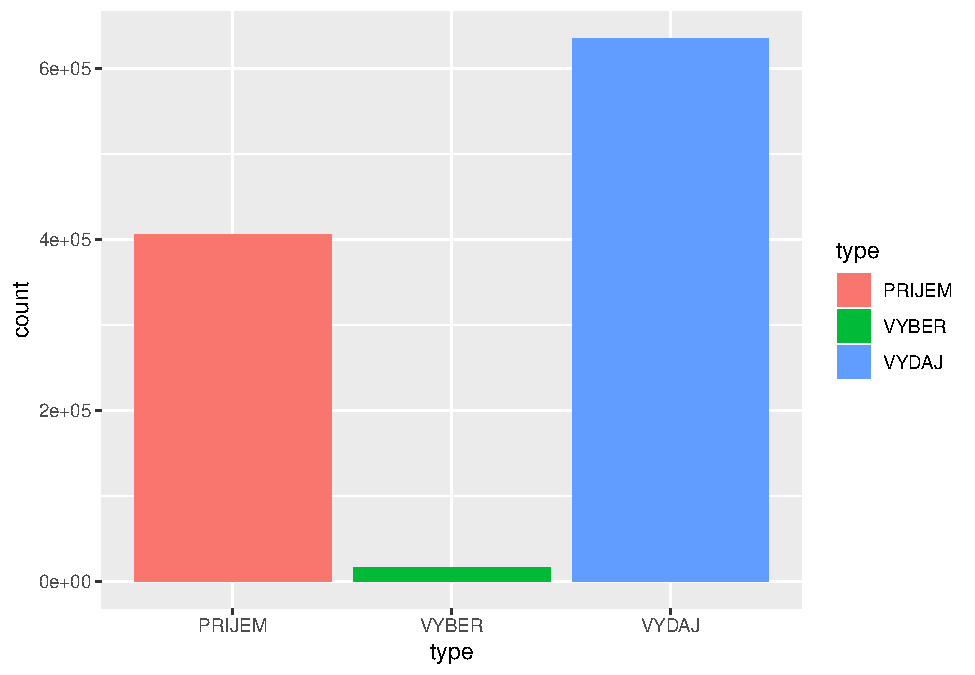
\includegraphics{analysis_gehrig_files/figure-latex/unnamed-chunk-6-1.pdf}

\hypertarget{trans-correction}{%
\paragraph{Trans correction}\label{trans-correction}}

\begin{Shaded}
\begin{Highlighting}[]
\NormalTok{trans_altered <-}\StringTok{ }\KeywordTok{alter_trans}\NormalTok{(trans)}
\NormalTok{account_altered <-}\StringTok{ }\KeywordTok{alter_account}\NormalTok{(account)}
\NormalTok{disp_altered <-}\StringTok{ }\KeywordTok{alter_disp}\NormalTok{(disp)}
\NormalTok{card_altered <-}\StringTok{ }\KeywordTok{alter_card}\NormalTok{(card)}
\NormalTok{loan_altered <-}\StringTok{ }\KeywordTok{alter_loan}\NormalTok{(loan)}
\end{Highlighting}
\end{Shaded}

\hypertarget{account-loan}{%
\paragraph{Account \& Loan}\label{account-loan}}

Hier wird gezeigt, dass jeder account nie mehr als eine loan besessen
hat.

\begin{Shaded}
\begin{Highlighting}[]
\NormalTok{account_loan_check <-}\StringTok{ }\ControlFlowTok{function}\NormalTok{(account_frame, loan_frame)\{}
\NormalTok{  account_loan <-}\StringTok{ }\NormalTok{dplyr}\OperatorTok{::}\KeywordTok{inner_join}\NormalTok{(account_frame, loan_frame, }\DataTypeTok{by =} \StringTok{'account_id'}\NormalTok{) }\OperatorTok
\StringTok{    }\NormalTok{dplyr}\OperatorTok{::}\KeywordTok{count}\NormalTok{(account_id) }\OperatorTok
\StringTok{    }\NormalTok{dplyr}\OperatorTok{::}\KeywordTok{select}\NormalTok{(n)}
  \KeywordTok{return}\NormalTok{(base}\OperatorTok{::}\KeywordTok{summary.data.frame}\NormalTok{(account_loan))}
\NormalTok{\}}

\KeywordTok{account_loan_check}\NormalTok{(account_altered, loan_altered)}
\end{Highlighting}
\end{Shaded}

\begin{verbatim}
##        n    
##  Min.   :1  
##  1st Qu.:1  
##  Median :1  
##  Mean   :1  
##  3rd Qu.:1  
##  Max.   :1
\end{verbatim}

\hypertarget{vermogen-pro-account}{%
\paragraph{Vermögen pro Account}\label{vermogen-pro-account}}

\begin{Shaded}
\begin{Highlighting}[]
\NormalTok{balance_account <-}\StringTok{ }\ControlFlowTok{function}\NormalTok{(trans_frame, }\DataTypeTok{min_date =}\NormalTok{ lowest_trans_date, }\DataTypeTok{max_date =}\NormalTok{ highest_trans_date)\{}
\NormalTok{  min_date <-}\StringTok{ }\KeywordTok{as.Date}\NormalTok{(min_date)}
\NormalTok{  max_date <-}\StringTok{ }\KeywordTok{as.Date}\NormalTok{(max_date)}
\NormalTok{  account_balance <-}\StringTok{ }\NormalTok{trans_frame }\OperatorTok\StringTok{ }
\StringTok{    }\NormalTok{dplyr}\OperatorTok{::}\KeywordTok{filter}\NormalTok{(trans_date }\OperatorTok{>=}\StringTok{ }\NormalTok{min_date }\OperatorTok{&}\StringTok{ }\NormalTok{trans_date }\OperatorTok{<=}\StringTok{ }\NormalTok{max_date) }\OperatorTok
\StringTok{    }\NormalTok{dplyr}\OperatorTok{::}\KeywordTok{group_by}\NormalTok{(account_id) }\OperatorTok
\StringTok{    }\NormalTok{dplyr}\OperatorTok{::}\KeywordTok{filter}\NormalTok{(trans_date }\OperatorTok{==}\StringTok{ }\KeywordTok{max}\NormalTok{(trans_date)) }\OperatorTok
\StringTok{    }\NormalTok{dplyr}\OperatorTok{::}\KeywordTok{filter}\NormalTok{(trans_id }\OperatorTok{==}\StringTok{ }\KeywordTok{max}\NormalTok{(trans_id)) }\OperatorTok
\StringTok{    }\NormalTok{dplyr}\OperatorTok{::}\KeywordTok{arrange}\NormalTok{(account_id)}
  \KeywordTok{return}\NormalTok{(account_balance)}
\NormalTok{\}}

\NormalTok{balance_distribution <-}\StringTok{ }\ControlFlowTok{function}\NormalTok{(trans_frame, }\DataTypeTok{min_date =}\NormalTok{ lowest_trans_date, }\DataTypeTok{max_date =}\NormalTok{ highest_trans_date, }\DataTypeTok{binwidth =} \DecValTok{2000}\NormalTok{)\{}
\NormalTok{  balances <-}\StringTok{ }\KeywordTok{balance_account}\NormalTok{(trans_frame, min_date, max_date)}
\NormalTok{  ggplot2}\OperatorTok{::}\KeywordTok{ggplot}\NormalTok{(}\DataTypeTok{data =}\NormalTok{ balances, }\KeywordTok{aes}\NormalTok{(balance)) }\OperatorTok{+}\StringTok{ }
\StringTok{  }\NormalTok{ggplot2}\OperatorTok{::}\KeywordTok{geom_density}\NormalTok{(}\KeywordTok{aes}\NormalTok{(}\DataTypeTok{y =}\NormalTok{..density..), }\DataTypeTok{fill =} \StringTok{'red'}\NormalTok{, }\DataTypeTok{alpha =} \FloatTok{0.85}\NormalTok{) }\OperatorTok{+}
\StringTok{  }\NormalTok{ggplot2}\OperatorTok{::}\KeywordTok{scale_x_continuous}\NormalTok{(}\DataTypeTok{labels =}\NormalTok{ scales}\OperatorTok{::}\NormalTok{comma) }\OperatorTok{+}
\StringTok{  }\NormalTok{ggplot2}\OperatorTok{::}\KeywordTok{labs}\NormalTok{(}\DataTypeTok{title =} \KeywordTok{paste0}\NormalTok{(}\StringTok{'Account Balance Distribution '}\NormalTok{, max_date), }\DataTypeTok{x =} \StringTok{'balance'}\NormalTok{, }\DataTypeTok{y =} \StringTok{'density'}\NormalTok{)}
\NormalTok{\}}

\NormalTok{b_acc <-}\StringTok{ }\KeywordTok{balance_account}\NormalTok{(trans_altered)}
\NormalTok{base}\OperatorTok{::}\KeywordTok{summary}\NormalTok{(b_acc}\OperatorTok{$}\NormalTok{balance)}
\end{Highlighting}
\end{Shaded}

\begin{verbatim}
##    Min. 1st Qu.  Median    Mean 3rd Qu.    Max. 
##  -25821   23075   38495   43809   60589  138317
\end{verbatim}

\begin{Shaded}
\begin{Highlighting}[]
\NormalTok{balance_dist <-}\StringTok{ }\KeywordTok{balance_distribution}\NormalTok{(trans_altered)}
\NormalTok{balance_dist}
\end{Highlighting}
\end{Shaded}

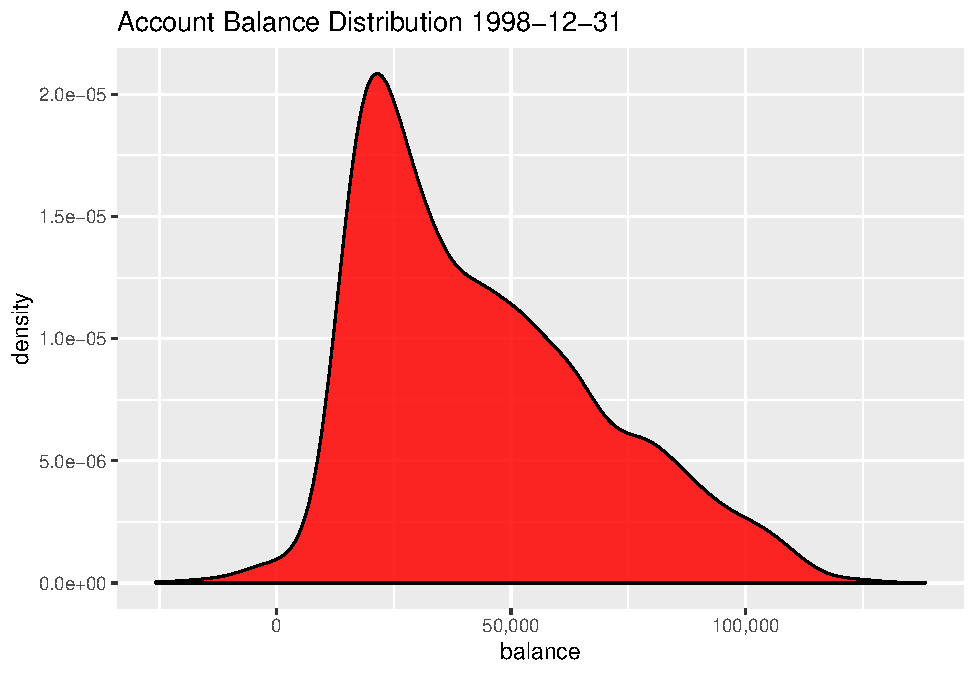
\includegraphics{analysis_gehrig_files/figure-latex/unnamed-chunk-9-1.pdf}

\hypertarget{vermogenverhaltnisse-der-bank}{%
\paragraph{Vermögenverhältnisse der
Bank}\label{vermogenverhaltnisse-der-bank}}

\begin{Shaded}
\begin{Highlighting}[]
\ControlFlowTok{for}\NormalTok{ (year }\ControlFlowTok{in}\NormalTok{ lowest_year}\OperatorTok{:}\NormalTok{highest_year) \{}
\NormalTok{  b_dist <-}\StringTok{ }\KeywordTok{balance_distribution}\NormalTok{(trans_altered, }\DataTypeTok{max_date =} \KeywordTok{ending_date}\NormalTok{(year))}
  \KeywordTok{print}\NormalTok{(b_dist)}
\NormalTok{\}}
\end{Highlighting}
\end{Shaded}

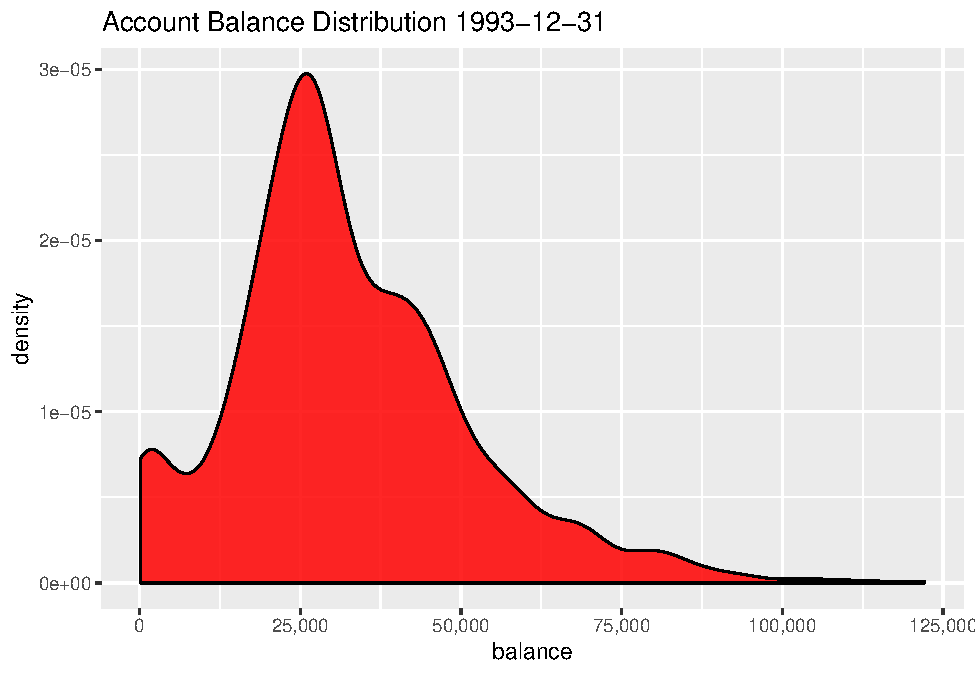
\includegraphics{analysis_gehrig_files/figure-latex/unnamed-chunk-10-1.pdf}
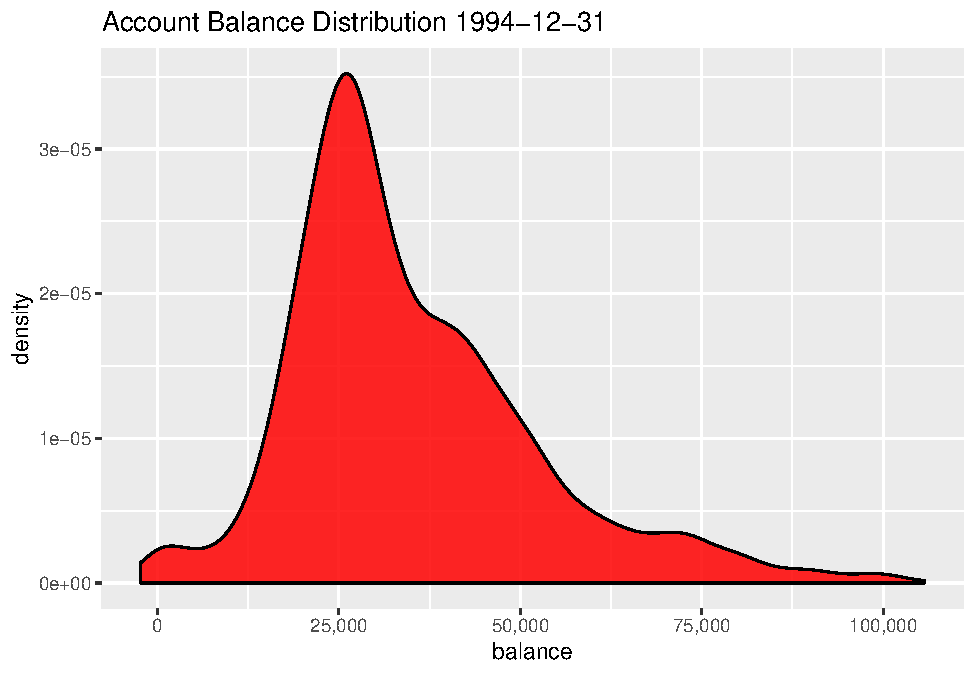
\includegraphics{analysis_gehrig_files/figure-latex/unnamed-chunk-10-2.pdf}
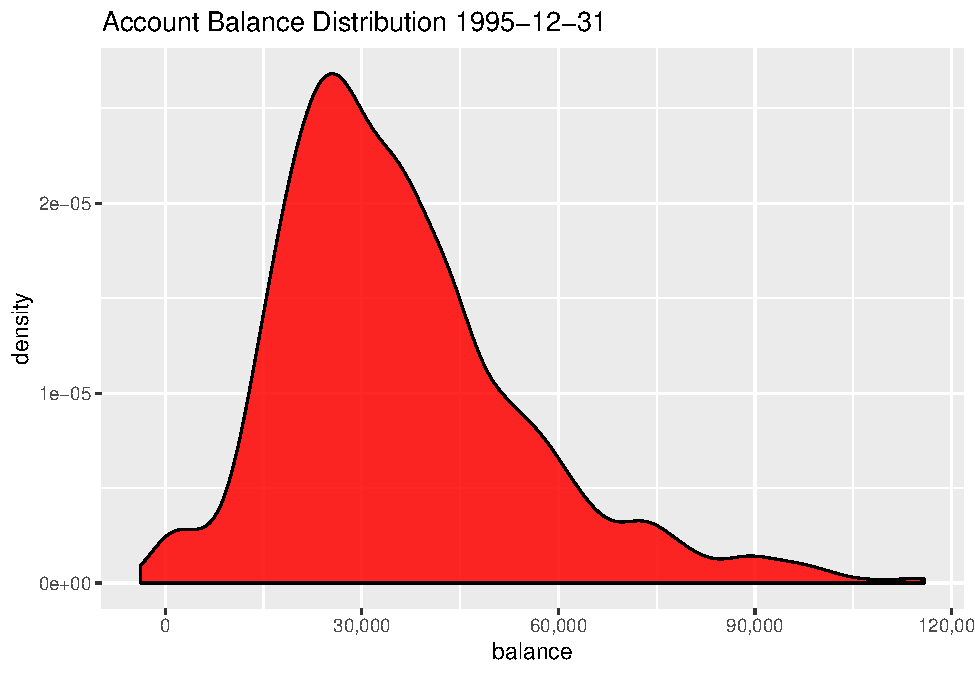
\includegraphics{analysis_gehrig_files/figure-latex/unnamed-chunk-10-3.pdf}
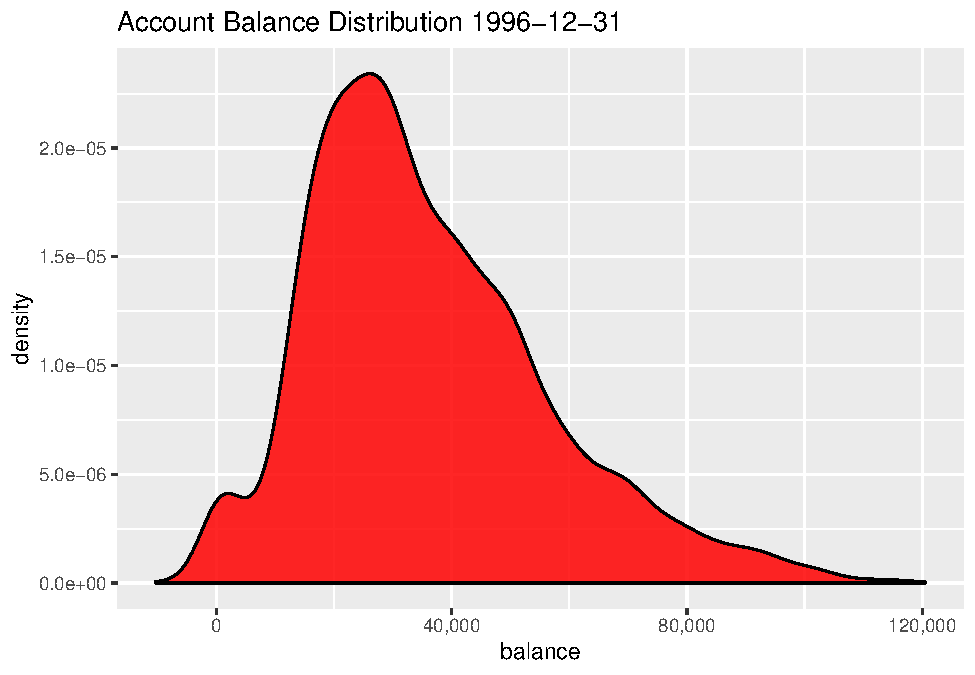
\includegraphics{analysis_gehrig_files/figure-latex/unnamed-chunk-10-4.pdf}
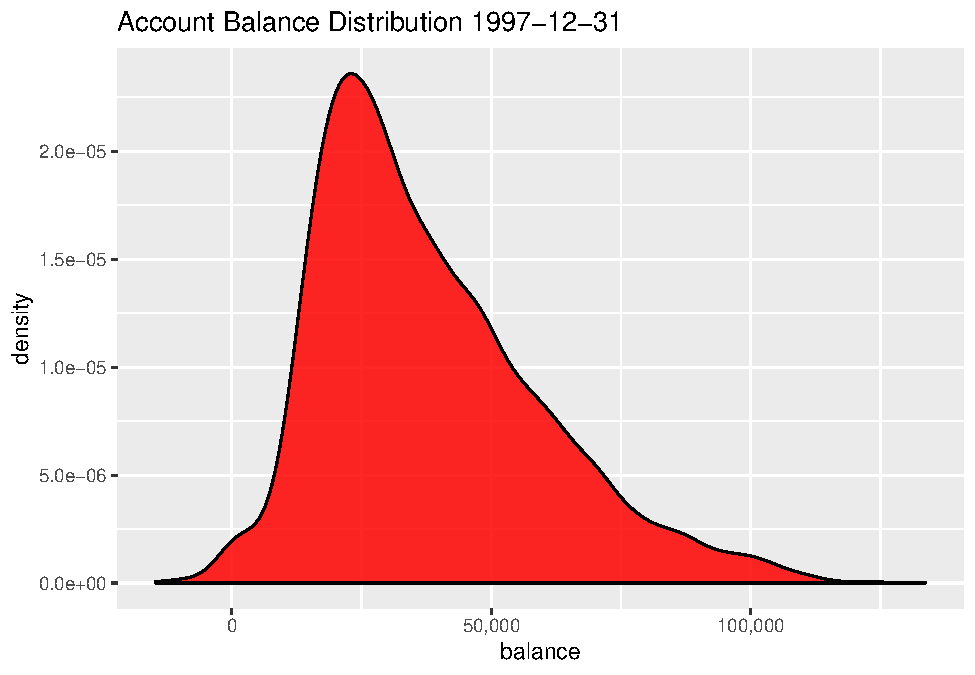
\includegraphics{analysis_gehrig_files/figure-latex/unnamed-chunk-10-5.pdf}
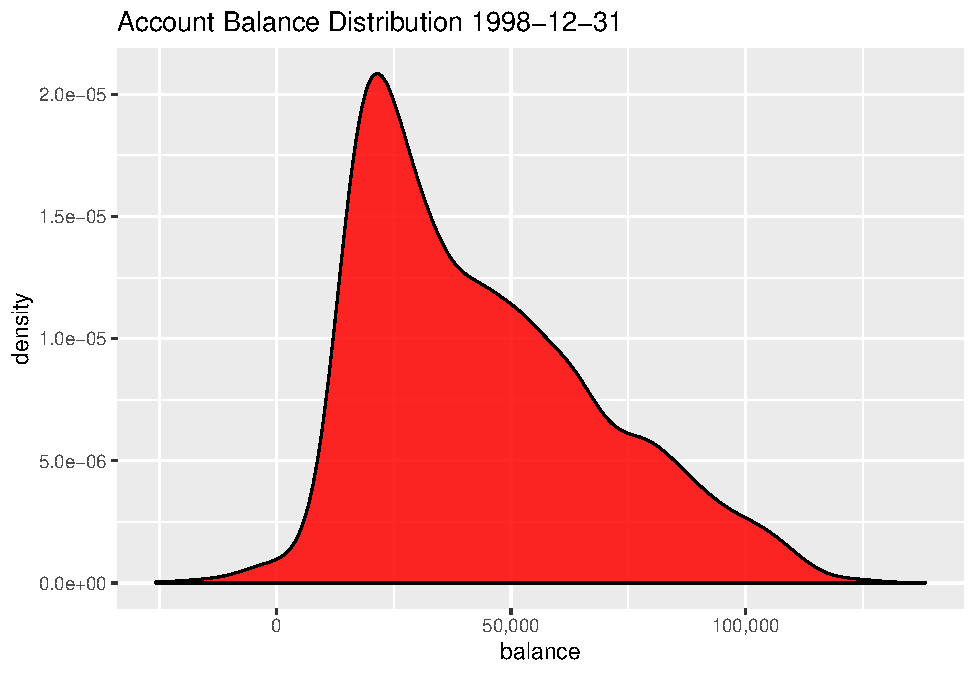
\includegraphics{analysis_gehrig_files/figure-latex/unnamed-chunk-10-6.pdf}

\hypertarget{card-ownership}{%
\paragraph{Card Ownership}\label{card-ownership}}

\begin{Shaded}
\begin{Highlighting}[]
\NormalTok{card_ownership <-}\StringTok{ }\ControlFlowTok{function}\NormalTok{(card_frame, disp_frame)\{}
\NormalTok{  ownership_frame <-}\StringTok{ }\NormalTok{card_frame }\OperatorTok
\StringTok{    }\NormalTok{dplyr}\OperatorTok{::}\KeywordTok{inner_join}\NormalTok{(disp_frame, }\DataTypeTok{by =} \StringTok{'disp_id'}\NormalTok{)}
  
\NormalTok{  ggplot2}\OperatorTok{::}\KeywordTok{ggplot}\NormalTok{(}\DataTypeTok{data =}\NormalTok{ ownership_frame) }\OperatorTok{+}\StringTok{ }
\StringTok{    }\NormalTok{ggplot2}\OperatorTok{::}\KeywordTok{geom_bar}\NormalTok{(}\DataTypeTok{mapping =} \KeywordTok{aes}\NormalTok{(}\DataTypeTok{x =}\NormalTok{ card_type, }\DataTypeTok{fill =}\NormalTok{ disp_type))}
\NormalTok{\}}

\KeywordTok{card_ownership}\NormalTok{(}\DataTypeTok{card_frame =}\NormalTok{ card_altered, }\DataTypeTok{disp_frame =}\NormalTok{ disp_altered)}
\end{Highlighting}
\end{Shaded}

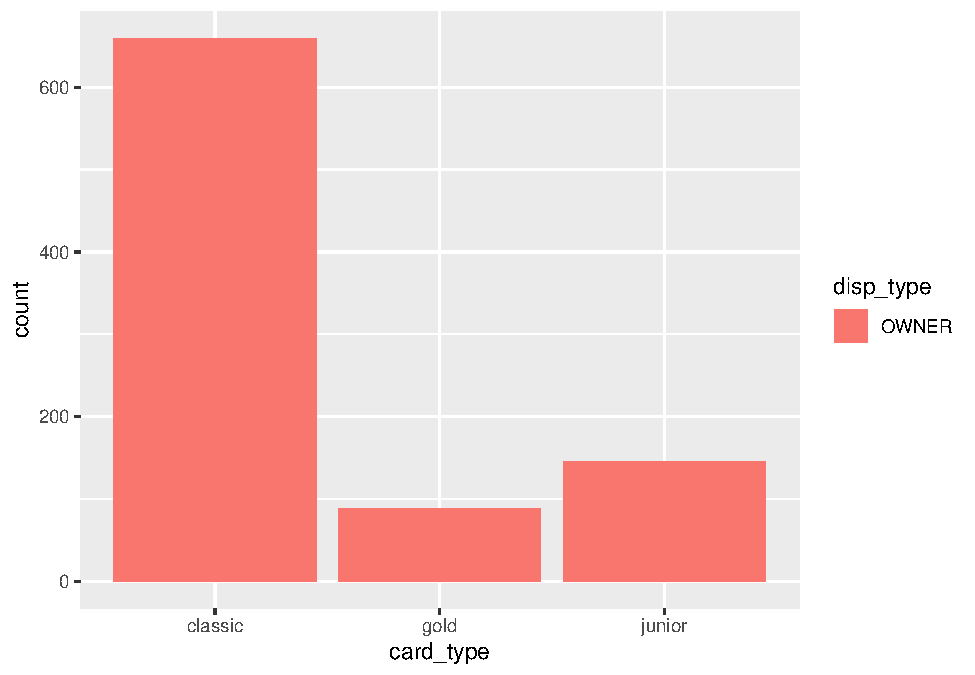
\includegraphics{analysis_gehrig_files/figure-latex/unnamed-chunk-11-1.pdf}

\hypertarget{jahrlicher-vermogensveranderung}{%
\paragraph{Jährlicher
Vermögensveränderung}\label{jahrlicher-vermogensveranderung}}

\begin{Shaded}
\begin{Highlighting}[]
\NormalTok{balance_delta <-}\StringTok{ }\ControlFlowTok{function}\NormalTok{(balances)\{}
  \KeywordTok{return}\NormalTok{(}\KeywordTok{c}\NormalTok{(}\OtherTok{NA}\NormalTok{, }\KeywordTok{diff}\NormalTok{(balances)))}
\NormalTok{\}}

\NormalTok{balance_delta_initial <-}\StringTok{ }\ControlFlowTok{function}\NormalTok{(balances)\{}
  \KeywordTok{return}\NormalTok{(}\KeywordTok{c}\NormalTok{(balances[}\DecValTok{1}\NormalTok{], }\KeywordTok{diff}\NormalTok{(balances)))}
\NormalTok{\}}

\NormalTok{balance_growth_end_of_years <-}\StringTok{ }\ControlFlowTok{function}\NormalTok{(trans_frame, }\DataTypeTok{with_initial_balance =} \OtherTok{FALSE}\NormalTok{)\{}
  \CommentTok{#' @description returns the yearly balance at end of year of each customer}
  
\NormalTok{  bal_grw <-}\StringTok{ }\NormalTok{trans_frame }\OperatorTok
\StringTok{    }\NormalTok{dplyr}\OperatorTok{::}\KeywordTok{mutate}\NormalTok{(}\DataTypeTok{year =} \KeywordTok{format}\NormalTok{(trans_date, }\StringTok{'%Y'}\NormalTok{)) }\OperatorTok
\StringTok{    }\NormalTok{dplyr}\OperatorTok{::}\KeywordTok{group_by}\NormalTok{(account_id, year) }\OperatorTok
\StringTok{    }\NormalTok{dplyr}\OperatorTok{::}\KeywordTok{filter}\NormalTok{(trans_date }\OperatorTok{==}\StringTok{ }\KeywordTok{max}\NormalTok{(trans_date)) }\OperatorTok
\StringTok{    }\NormalTok{dplyr}\OperatorTok{::}\KeywordTok{filter}\NormalTok{(trans_id }\OperatorTok{==}\StringTok{ }\KeywordTok{max}\NormalTok{(trans_id)) }\OperatorTok
\StringTok{    }\NormalTok{dplyr}\OperatorTok{::}\KeywordTok{arrange}\NormalTok{(account_id, trans_date)}
   
  \ControlFlowTok{if}\NormalTok{ (with_initial_balance)\{}
\NormalTok{    bal_grw}\OperatorTok{$}\NormalTok{balance_delta <-}\StringTok{ }\KeywordTok{as.numeric}\NormalTok{(}\KeywordTok{unlist}\NormalTok{(}\KeywordTok{by}\NormalTok{(bal_grw}\OperatorTok{$}\NormalTok{balance, bal_grw}\OperatorTok{$}\NormalTok{account_id, balance_delta_initial)))}
\NormalTok{  \}}\ControlFlowTok{else}\NormalTok{\{}
\NormalTok{    bal_grw}\OperatorTok{$}\NormalTok{balance_delta <-}\StringTok{ }\KeywordTok{as.numeric}\NormalTok{(}\KeywordTok{unlist}\NormalTok{(}\KeywordTok{by}\NormalTok{(bal_grw}\OperatorTok{$}\NormalTok{balance, bal_grw}\OperatorTok{$}\NormalTok{account_id, balance_delta)))}
\NormalTok{  \}}
  \KeywordTok{return}\NormalTok{(bal_grw)}
\NormalTok{\}}

\NormalTok{customer_balance_change_estimation <-}\StringTok{ }\ControlFlowTok{function}\NormalTok{(trans_frame, }\DataTypeTok{without_initial_balance =} \OtherTok{FALSE}\NormalTok{, }\DataTypeTok{min_date =}\NormalTok{ lowest_trans_date, }\DataTypeTok{max_date =}\NormalTok{ highest_trans_date, }\DataTypeTok{join_data_frame =} \OtherTok{NA}\NormalTok{)\{}
  \CommentTok{#' @description returns the estimated income and expenses, total and monthly, from each customer. In addition, the already jointed data frame 'card', 'disp' & 'account' can be given to get the above mentioned figures at the time of the customer's receipt of their credit card.}
  
\NormalTok{  cust_bal_ch <-}\StringTok{ }\NormalTok{trans_frame}
  
  \ControlFlowTok{if}\NormalTok{(without_initial_balance)\{}\CommentTok{#filters opening balance if one is interested just in the estimated income}
\NormalTok{    cust_bal_ch <-}\StringTok{ }\NormalTok{cust_bal_ch }\OperatorTok
\StringTok{      }\NormalTok{dplyr}\OperatorTok{::}\KeywordTok{group_by}\NormalTok{(account_id) }\OperatorTok
\StringTok{      }\NormalTok{dplyr}\OperatorTok{::}\KeywordTok{filter}\NormalTok{(trans_date }\OperatorTok{!=}\StringTok{ }\KeywordTok{min}\NormalTok{(trans_date))}
\NormalTok{  \}}
  
  \ControlFlowTok{if}\NormalTok{(}\KeywordTok{is.na}\NormalTok{(join_data_frame))\{}
\NormalTok{  cust_bal_ch <-}\StringTok{ }\NormalTok{cust_bal_ch }\OperatorTok
\StringTok{    }\NormalTok{dplyr}\OperatorTok{::}\KeywordTok{filter}\NormalTok{(trans_date }\OperatorTok{>=}\StringTok{ }\NormalTok{min_date }\OperatorTok{&}\StringTok{ }\NormalTok{trans_date }\OperatorTok{<=}\StringTok{ }\NormalTok{max_date) }\OperatorTok
\StringTok{    }\NormalTok{dplyr}\OperatorTok{::}\KeywordTok{group_by}\NormalTok{(account_id, trans_type) }\OperatorTok
\StringTok{    }\NormalTok{dplyr}\OperatorTok{::}\KeywordTok{summarise}\NormalTok{(}\DataTypeTok{balance_change =} \KeywordTok{sum}\NormalTok{(trans_amount))}
\NormalTok{  \}}\ControlFlowTok{else}\NormalTok{\{}
\NormalTok{    cust_bal_ch <-}\StringTok{ }\NormalTok{cust_bal_ch }\OperatorTok
\StringTok{    }\NormalTok{dplyr}\OperatorTok{::}\KeywordTok{inner_join}\NormalTok{(join_data_frame, }\DataTypeTok{by =} \StringTok{'account_id'}\NormalTok{) }\OperatorTok
\StringTok{    }\NormalTok{dplyr}\OperatorTok{::}\KeywordTok{group_by}\NormalTok{(account_id) }\OperatorTok
\StringTok{    }\NormalTok{dplyr}\OperatorTok{::}\KeywordTok{filter}\NormalTok{(trans_date }\OperatorTok{<}\StringTok{ }\NormalTok{issued) }\OperatorTok
\StringTok{    }\NormalTok{dplyr}\OperatorTok{::}\KeywordTok{filter}\NormalTok{(trans_date }\OperatorTok{>=}\StringTok{ }\NormalTok{min_date }\OperatorTok{&}\StringTok{ }\NormalTok{trans_date }\OperatorTok{<=}\StringTok{ }\NormalTok{max_date) }\OperatorTok
\StringTok{    }\NormalTok{dplyr}\OperatorTok{::}\KeywordTok{group_by}\NormalTok{(account_id, trans_type, card_type) }\OperatorTok\StringTok{ }\CommentTok{#including card_type}
\StringTok{    }\NormalTok{dplyr}\OperatorTok{::}\KeywordTok{summarise}\NormalTok{(}\DataTypeTok{balance_change =} \KeywordTok{sum}\NormalTok{(trans_amount))}
\NormalTok{  \}}
  
\NormalTok{  cust_bal_ch}\OperatorTok{$}\NormalTok{balance_delta <-}\StringTok{ }\NormalTok{(}\KeywordTok{as.numeric}\NormalTok{(}\KeywordTok{unlist}\NormalTok{(}\KeywordTok{by}\NormalTok{(cust_bal_ch}\OperatorTok{$}\NormalTok{balance_change, cust_bal_ch}\OperatorTok{$}\NormalTok{account_id, balance_delta)))}\OperatorTok{*-}\DecValTok{1}\NormalTok{)}
  
\NormalTok{  cust_bal_ch <-}\StringTok{ }\NormalTok{trans_frame }\OperatorTok
\StringTok{    }\NormalTok{dplyr}\OperatorTok{::}\KeywordTok{filter}\NormalTok{(trans_date }\OperatorTok{>=}\StringTok{ }\NormalTok{min_date }\OperatorTok{&}\StringTok{ }\NormalTok{trans_date }\OperatorTok{<=}\StringTok{ }\NormalTok{max_date) }\OperatorTok
\StringTok{    }\NormalTok{dplyr}\OperatorTok{::}\KeywordTok{group_by}\NormalTok{(account_id) }\OperatorTok
\StringTok{    }\NormalTok{dplyr}\OperatorTok{::}\KeywordTok{summarise}\NormalTok{(}\DataTypeTok{duration_month =}\NormalTok{ (zoo}\OperatorTok{::}\KeywordTok{as.yearmon}\NormalTok{(}\KeywordTok{max}\NormalTok{(trans_date)) }\OperatorTok{-}\StringTok{ }\NormalTok{zoo}\OperatorTok{::}\KeywordTok{as.yearmon}\NormalTok{(}\KeywordTok{min}\NormalTok{(trans_date))) }\OperatorTok{*}\StringTok{ }\DecValTok{12} \OperatorTok{+}\StringTok{ }\DecValTok{1}\NormalTok{) }\OperatorTok\StringTok{ }\CommentTok{#diff num of months}
\StringTok{    }\NormalTok{dplyr}\OperatorTok{::}\KeywordTok{inner_join}\NormalTok{(cust_bal_ch, }\DataTypeTok{by =} \StringTok{'account_id'}\NormalTok{) }\OperatorTok
\StringTok{    }\NormalTok{dplyr}\OperatorTok{::}\KeywordTok{mutate}\NormalTok{(}\DataTypeTok{monthly_change =}\NormalTok{ balance_change }\OperatorTok{/}\StringTok{ }\NormalTok{duration_month) }\OperatorTok
\StringTok{    }\NormalTok{dplyr}\OperatorTok{::}\KeywordTok{mutate}\NormalTok{(}\DataTypeTok{monthly_balance_delta_change =}\NormalTok{ balance_delta }\OperatorTok{/}\StringTok{ }\NormalTok{duration_month)}
  
  \KeywordTok{return}\NormalTok{(cust_bal_ch)}
\NormalTok{\}}

\KeywordTok{customer_balance_change_estimation}\NormalTok{(}\DataTypeTok{trans_frame =}\NormalTok{ trans_altered)}
\end{Highlighting}
\end{Shaded}

\begin{verbatim}
## # A tibble: 9,000 x 7
##    account_id duration_month trans_type balance_change balance_delta
##         <int>          <dbl> <chr>               <int>         <dbl>
##  1          1            46  PRIJEM             194322            NA
##  2          1            46  VYDAJ              180870         13452
##  3          2            71. PRIJEM            1597055            NA
##  4          2            71. VYDAJ             1554459         42596
##  5          3            18. PRIJEM             173062            NA
##  6          3            18. VYDAJ              121968         51094
##  7          4            35. PRIJEM             192349            NA
##  8          4            35. VYDAJ              158637         33712
##  9          5            20. PRIJEM              97489            NA
## 10          5            20. VYDAJ               69402         28087
## # ... with 8,990 more rows, and 2 more variables: monthly_change <dbl>,
## #   monthly_balance_delta_change <dbl>
\end{verbatim}

\hypertarget{card-balance-change-correlation}{%
\paragraph{Card \& Balance
Change-Correlation}\label{card-balance-change-correlation}}

\begin{Shaded}
\begin{Highlighting}[]
\NormalTok{card_balance_change_correlation <-}\StringTok{ }\ControlFlowTok{function}\NormalTok{(trans_frame, account_frame, disp_frame, card_frame)\{}
\NormalTok{  prep_frame <-}\StringTok{ }\NormalTok{card_frame }\OperatorTok
\StringTok{    }\NormalTok{dplyr}\OperatorTok{::}\KeywordTok{inner_join}\NormalTok{(disp_frame, }\DataTypeTok{by =} \StringTok{'disp_id'}\NormalTok{) }\OperatorTok
\StringTok{    }\NormalTok{dplyr}\OperatorTok{::}\KeywordTok{inner_join}\NormalTok{(account_frame, }\DataTypeTok{by =} \StringTok{'account_id'}\NormalTok{)}
  
\NormalTok{  estimated_balance_change_frame <-}\StringTok{ }\KeywordTok{customer_balance_change_estimation}\NormalTok{(}\DataTypeTok{trans_frame =}\NormalTok{ trans_frame, }\DataTypeTok{join_data_frame =}\NormalTok{ prep_frame)}
  
  \KeywordTok{return}\NormalTok{(estimated_balance_change_frame)}
\NormalTok{\}}

\KeywordTok{card_balance_change_correlation}\NormalTok{(trans_altered, account_altered, disp_altered, card_altered)}
\end{Highlighting}
\end{Shaded}

\begin{verbatim}
## Warning in if (is.na(join_data_frame)) {: Bedingung hat Länge > 1 und nur
## das erste Element wird benutzt
\end{verbatim}

\begin{verbatim}
## # A tibble: 1,784 x 8
##    account_id duration_month trans_type card_type balance_change
##         <int>          <dbl> <chr>      <chr>              <int>
##  1          7            26. PRIJEM     gold              572689
##  2          7            26. VYDAJ      gold              501690
##  3         14            26. PRIJEM     classic           263177
##  4         14            26. VYDAJ      classic           214784
##  5         33            65. PRIJEM     gold              621303
##  6         33            65. VYDAJ      gold              563348
##  7         34            64  PRIJEM     classic          2148185
##  8         34            64  VYDAJ      classic          2105856
##  9         43            55  PRIJEM     junior            290502
## 10         43            55  VYDAJ      junior            224324
## # ... with 1,774 more rows, and 3 more variables: balance_delta <dbl>,
## #   monthly_change <dbl>, monthly_balance_delta_change <dbl>
\end{verbatim}

\hypertarget{transaktionstype-analyse}{%
\paragraph{Transaktionstype-analyse}\label{transaktionstype-analyse}}

\begin{Shaded}
\begin{Highlighting}[]
\NormalTok{analyze_transactions <-}\StringTok{ }\ControlFlowTok{function}\NormalTok{(trans_frame)\{}
\NormalTok{  frame <-}\StringTok{ }\NormalTok{trans_frame }\OperatorTok
\StringTok{    }\NormalTok{dplyr}\OperatorTok{::}\KeywordTok{arrange}\NormalTok{(account_id, trans_date, }\KeywordTok{desc}\NormalTok{(trans_id)) }\OperatorTok
\StringTok{    }\NormalTok{dplyr}\OperatorTok{::}\KeywordTok{group_by}\NormalTok{(account_id) }\OperatorTok
\StringTok{    }\NormalTok{dplyr}\OperatorTok{::}\KeywordTok{mutate}\NormalTok{(}\DataTypeTok{balance_diff =}\NormalTok{ (balance }\OperatorTok{-}\StringTok{ }\NormalTok{dplyr}\OperatorTok{::}\KeywordTok{lag}\NormalTok{(balance))) }\OperatorTok
\StringTok{    }\NormalTok{dplyr}\OperatorTok{::}\KeywordTok{filter}\NormalTok{(}\KeywordTok{round2}\NormalTok{(}\KeywordTok{abs}\NormalTok{(balance_diff), }\DecValTok{0}\NormalTok{) }\OperatorTok{==}\StringTok{ }\NormalTok{trans_amount) }\OperatorTok\StringTok{ }\CommentTok{#ensures to just consider 100% correct calculated balance_diff}
\StringTok{    }\NormalTok{dplyr}\OperatorTok{::}\KeywordTok{filter}\NormalTok{(trans_type }\OperatorTok{==}\StringTok{ 'PRIJEM'}\NormalTok{) }\OperatorTok
\StringTok{    }\NormalTok{dplyr}\OperatorTok{::}\KeywordTok{filter}\NormalTok{(balance_diff }\OperatorTok{<=}\StringTok{ }\DecValTok{0}\NormalTok{)}
  
  \KeywordTok{return}\NormalTok{(frame)}
\NormalTok{\}}

\KeywordTok{analyze_transactions}\NormalTok{(trans_altered)}
\end{Highlighting}
\end{Shaded}

\begin{verbatim}
## # A tibble: 631 x 11
## # Groups:   account_id [159]
##    trans_id account_id trans_date trans_type operation trans_amount balance
##       <int>      <int> <date>     <chr>      <chr>            <int>   <dbl>
##  1  3445002         19 1995-04-30 PRIJEM     <NA>                47  16186.
##  2  3445007         19 1995-09-30 PRIJEM     <NA>                98  16840.
##  3  3445009         19 1995-11-30 PRIJEM     <NA>                76   3669.
##  4  3445013         19 1996-03-31 PRIJEM     <NA>                84  16246.
##  5  3445020         19 1996-09-30 PRIJEM     <NA>                92  22102.
##  6  3445021         19 1996-10-31 PRIJEM     <NA>                76  19872.
##  7  3445028         19 1997-05-31 PRIJEM     <NA>                12   7898.
##  8  3445109        103 1997-05-31 PRIJEM     <NA>               274  62949.
##  9  3445110        103 1997-06-30 PRIJEM     <NA>               171  45423.
## 10  3445111        103 1997-07-31 PRIJEM     <NA>               276  97315.
## # ... with 621 more rows, and 4 more variables: k_symbol <chr>,
## #   bank <chr>, account <dbl>, balance_diff <dbl>
\end{verbatim}

\#\texttt{\{r\ child\ =\ \textquotesingle{}../footer.Rmd\textquotesingle{}\}\ \#}


\end{document}
